\documentclass[../../main.tex]{subfiles}
\begin{document}

\begin{flushright}
  \footnotesize\textit{【自動文字起こし・要確認】}
\end{flushright}

{\bf [解]}
$L:y=2x\ (0\le x\le1)$である．よって，
\begin{align}
  x^2+ax+b=2x\quad(0\le x\le1)
\end{align}
が解を持てば良い．$f(x)=x^2+(a-2)x+b$とおく．

\underline{$1^\circ$ 区間内に$1$つ}
\begin{align}
  f(0)f(1)\le0\iff b(a+b-1)\le0
\end{align}

\underline{$2^\circ$ 区間内に$2$つ（重解含む）}
\begin{align}
  \text{判別式：}&(a-2)^2-4b\ge0\\
  \text{端点：}&f(0)\ge0，\ f(1)\ge0\\
  \text{軸：}&0\le\dfrac{2-a}{2}\le1
\end{align}
\begin{align}
  \iff\quad b\le\dfrac{1}{4}(a-2)^2，\qquad b\ge0，\ a+b-1\ge0，\qquad0\le a\le2
\end{align}

以上を図示して，下図斜線部（境界含む）．

\begin{figure}[htb]
  \centering
  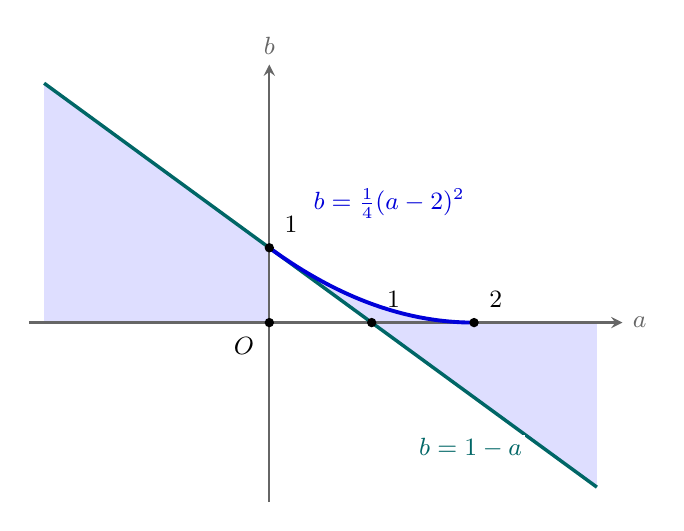
\begin{tikzpicture}[x=1.3cm, y=0.95cm, >=stealth,
    every node/.style={font=\small}]
    % a<0 と a>2 では f(0)f(1)\leq0、0\leq a\leq2 では判別式の条件も使う。
    \fill[blue!13] (-2.2,0) -- (0,0) -- (0,1) -- (-2.2,3.2) -- cycle;
    \fill[blue!13] (0,1) plot[domain=0:2, samples=80]
    (\x,{0.25*(\x-2)^2}) -- (2,-1) -- cycle;
    \fill[blue!13] (2,0) -- (3.2,0) -- (3.2,-2.2) -- (2,-1) -- cycle;
    \draw[->, thick, gray!80!black] (-2.35,0) -- (3.45,0) node[right] {$a$};
    \draw[->, thick, gray!80!black] (0,-2.4) -- (0,3.45) node[above] {$b$};
    \draw[line width=1.25pt, teal!80!black] (-2.2,3.2) -- (3.2,-2.2);
    \draw[line width=1.4pt, blue!85!black]
    plot[domain=0:2, samples=80] (\x,{0.25*(\x-2)^2});
    \node[circle, fill, inner sep=1.2pt] at (0,0) {}; \node[below left=2pt] at (0,0) {$O$};
    \node[circle, fill, inner sep=1.2pt] at (1,0) {}; \node[above right=2pt] at (1,0) {$1$};
    \node[circle, fill, inner sep=1.2pt] at (2,0) {}; \node[above right=2pt] at (2,0) {$2$};
    \node[circle, fill, inner sep=1.2pt] at (0,1) {}; \node[above right=2pt] at (0,1) {$1$};
    \node[blue!85!black, fill=white, inner sep=1pt, above right]
    at (0.4,1.35) {$b=\frac{1}{4}(a-2)^2$};
    \node[teal!80!black, fill=white, inner sep=1pt, below left]
    at (2.5,-1.5) {$b=1-a$};
  \end{tikzpicture}
  \caption{条件を満たす$(a,b)$の範囲（着色部，境界含む）}
\end{figure}

\newpage

\end{document}
